\documentclass[../../main.tex]{subfiles}
\begin{document}

\section{Definition und Beispiele abelscher Gruppen}

\begin{df}\label{2.1.1}
Eine \emph{abelsche Gruppe}\index{abelsche Gruppe@{\bf abelsche Gruppe}} ist ein geordnetes Paar (d.h. 2-Tupel) $(G,+)$, wobei $G$ eine Menge ist und $+:G\times G\rightarrow G$ eine Abbildung (meist infix geschrieben, d.h. man schreibt $a+b$ statt $+(a,b))$ mit folgenden Eigenschaften:
\begin{itemize}
\item[(K)] $\forall a,b\in G : a+b = b+a $ \qquad{\small "`kommutativ"'}\index{kommutativ@{\bf kommutativ}}
\item[(A)] $\forall a,b,c\in G: a+ (b+c) = (a+b)+c$ \qquad{\small "`assoziativ"'}\index{assoziativ@{\bf assoziativ}}
\item[(N)] $\exists e \in G : \forall a\in G: a+e = a$ \qquad
{\small"`neutrales Element"'}\index{neutrales Element@{\bf neutrales Element}}

\smallskip\noindent
\emph{Anmerkung:} sind $e,e'\in G$ neutral, d.h. $\forall a\in G: a+e=a=a+e'$, so gilt $e=e'$, denn es gilt
$e'=e'+e\overset{\text{(K)}} = e+e' = e$.
Daher gibt es \emph{genau} ein $e\in G$ mit $\forall e\in G: a+e=a$ und man bezeichnet dieses $e$ als das \emph{neutrale Element} der Gruppe und schreibt dafür $0$ statt $e$.
\item[(I)] $\forall a\in G : \exists b\in G: a+b=0$ \qquad{\small"`inverse Elemente"'}\index{inverse Elemente@{\bf inverse Elemente}}
\end{itemize}
\end{df}

\begin{bem}\label{2.1.2}
\begin{enumerate}[\normalfont(a)]
\item Ist $(G,+)$ eine abelsche Gruppe, so nennt man $G$ die \emph{zugrundeliegende} (oder \emph{Träger-})\emph{Menge}\index{abelsche Gruppe@{\bf abelsche Gruppe}!zugrundeliegende Menge/ Trägermenge} und $+$ die (Gruppen-)\emph{Addition} von $(G,+)$.
\item Sei $(G,+)$ eine abelsche Gruppe und $a\in G$. Seien $b,b'$ invers zu $a$, d.h. $a+b=0=a+b'$. Dann gilt $b=b'$, denn es gilt
$$b\overset{\text{(N)}} = b+0 = b+(a+b') \overset{\text{(A)}} = (b+a)+b' \overset{\text{(K)}} = (a+b)+b' = 0+b' \overset{\text{(K)}}= b'+0 \overset{\text{(N)}}= b'$$
Daher ist zu jedem $a\in G$ das dazu inverse Element eindeutig bestimmt und wir führen die Abbildung
\[-:G\rightarrow G, a\mapsto b\text{ falls }a+b=0\]
ein. Statt $-(a)$ schreibt man oft $-a$ und statt $a+(-b)$ schreibt man oft $a-b$.
\item (N) und (I) kann man nun wie folgt schreiben:
\begin{itemize}
\item[(N)] $\forall a\in G:a+0=a$
\item[(I)] $\forall a\in G:a+(-a)=0$
\end{itemize}
\item Statt $+$ kann man natürlich auch andere Symbole benutzen. Zur gleichzeitigen Betrachtung mehrerer Gruppen schreibt man manchmal $(G,+_G)$, $(H,+_H)$, usw. und dann entsprechend $0_G, 0_H, -_G, -_H$. Da aus dem Kontext oft klar ist, ob $+_G$ oder $+_H$ gemeint ist, schreibt man oft schlampig $+$ sowohl für $+_G$ als auch für $+_H$. Manchmal schreibt man auch $\begin{Bmatrix}ab=a\cdot b\\1\\a^{-1}\end{Bmatrix}$ statt $\begin{Bmatrix}a+b\\0 \\ -a \end{Bmatrix}$, z.B. sind $(\R\setminus \left\{0\right\},\cdot), (\R_{>0},\cdot)$ und $(\left\{-1,1\right\},\cdot)$ jeweils mit der Multiplikation reeller Zahlen aus der jeweils zugrundeliegenden Menge abelsche Gruppen.
\item Statt "`$(G,+)$ ist abelsche Gruppe"' schreibt man oft auch "`$G$ ist additiv geschriebene abelsche Gruppe"' oder nur "`$G$ ist abelsche Gruppe"' (obwohl $G$ nur die Trägermenge (siehe (a)) einer abelschen Gruppe ist). Statt "`$(G,\cdot)$ ist abelsche Gruppe"' schreibt man oft auch "`$G$ ist multiplikativ geschriebene abelsche Gruppe"'.
\end{enumerate}
\end{bem}

\begin{bsp}\label{2.1.3}
\begin{enumerate}[\normalfont(a)]
\item Ist $a$ ein mathematisches Objekt, so ist$(\left\{a\right\},+)$ mit
$$+:\left\{a\right\}\times\left\{a\right\}\rightarrow \left\{a\right\}, (a,a)\mapsto a$$
eine abelsche Gruppe, in der gilt:
$$a+a = a, 0=a, \text{ und } -a=a$$
Dies ist die einzige abelsche Gruppe mit Trägermenge $\left\{a\right\}$.
\item Die leere Menge ist keine Trägermenge einer abelschen Gruppe wegen $(N)$.
\item Ist $(G,+)$ eine zweielementige abelsche Gruppe, so gibt es $a\in G$ mit $G=\left\{0,a\right\}, a\neq 0$ und aus $(I)$ folgt $a+0=0$ oder $a+a=0$.\\
Aus $a+0=0$ würde aber $a\overset{(N)}= a+0=0$ folgen im Widerspruch zu $a\neq 0$. Also gilt $a+a=0$. Mit $(K)$ und $(N)$ erhält man die Addition $+$ von $(G,+)$ in Form einer \emph{Additionstabelle}:
\begin{table}[h]
\centering
\begin{tabular}{c|cc}
 $+$ & $0$ & $a$ \\\hline
 $0$ & $0$ & $a$ \\
 $a$ & $a$ & $0$
\end{tabular}
\end{table}\\
\emph{Vorsicht!} Damit ist nicht gezeigt, dass es eine zweielementige abelsche Gruppe gibt. Es ist nur gezeigt, dass jede zweielementige abelsche Gruppe so ausschaut.\\
\textbf{Übung:} Zeige, dass durch diese Tabelle eine abelsche Gruppe definiert wird.
\item Ist $(G,+)$ eine dreielementige abelsche Gruppe, so gibt es $a,b\in G$ mit $G=\left\{0,a,b\right\}$ und $0,a,b$ paarweise verschieden.\\
Wäre $a+b=a$, so folgte 
$$b\overset{(N)}=b+0\overset{(I)}= b+(a+(-a))\overset{(A)}=(b+a)+(-a)\overset{(K)}=(a+b)+(-a)=a+(-a)\overset{(I)}=0 ~\lightning.$$
Also gilt $a+b\neq a$. Analog folgt $a+b\neq b$. Daher muss $a+b=0$ gelten, also ist $b=-a$. Wäre $a+a=0$, so folgte $a=-a=b ~\lightning$. Wäre $a+a=a$, so folgte $a\overset{(N)}=a+0\overset{(I)}= a+(a+(-a))\overset{(A)}=(a+a)+(-a)=a+(-a)\overset{(I)}=0 ~\lightning$. Also muss $a+a=b$ gelten. Analog zeigt man $b+b=a$. Mit $(N)$ und $(K)$ erhält man die Additionstabelle von $(G,+)$:
\begin{table}[h]
\centering
\begin{tabular}{c|ccc}
 $+$ & $0$ & $a$ & $b$ \\\hline
 $0$ & $0$ & $a$ & $b$ \\
 $a$ & $a$ & $b$ & $0$ \\
 $b$ & $b$ & $0$ & $a$
\end{tabular} 
\begin{tabular}{c}
\emph{Vorsicht!} [$\rightarrow$ (c)]
\end{tabular}
\end{table}
\item Sei $A$ eine Menge. Dann ist $(\Pow(A),+)$ mit 
\begin{align*}
+:\Pow(A)\times \Pow(A) &\rightarrow\Pow(A)\\
(B,C) & \mapsto B\hspace{-2em}\underbrace{\Delta}_{\over{\text{"`symmetrische}}{\text{Mengendifferenz"'}}}\hspace{-2em}
C := (B\setminus C)\cup (C\setminus B)
\end{align*}\index{Menge@{\bf Menge}!symmetrische Differenz ($\Delta$)}
eine abelsche Gruppe mit $0=\emptyset$ und $-B = B$ für $B\in\Pow(A)$.
\item $\Z,\Q,\R,\left\{5n\mid n\in\Z\right\},\left\{\frac{n}{2}\mid n\in\Z\right\}$ bilden zusammen mit der gewöhnlichen Addition auf ihnen jeweils eine abelsche Gruppe, nicht jedoch $\N$ oder $\N_0$.\\
$\left\{0\right\}, \left\{1\right\}, \left\{-1,1\right\}, \Q\setminus\left\{0\right\}, \Q_{>0}, \R\setminus\left\{0\right\}, \R_{>0}$ bilden zusammen mit der gewöhnlichen Multiplikation auf ihnen jeweils eine (multiplikativ geschriebene [$\rightarrow$ \ref{2.1.2} (d)]) abelsche Gruppe, nicht jedoch $\left\{0,1\right\},\Q$ oder $\R$.
\end{enumerate}
\end{bsp}

\begin{pro}\label{2.1.4}
Sei $G$ eine abelsche Gruppe {\rm[$\rightarrow$ \ref{2.1.2} (e)]}. Dann gilt für alle $a,b\in G$:
$$-(-a)=a\text{ und }-(a+b)=(-a)+(-b)$$
\end{pro}
\begin{proof}
Seien $a,b\in G$. Um $-(-a)=a$ zu zeigen, genügt es, $-a+a=0$ zu zeigen [$\rightarrow$ \ref{2.1.2} (b)], was aber sofort aus $(I)$ und $(K)$ folgt. Um $-(a+b)=(-a)+(-b)$ zu zeigen, ist $(a+b)+((-a)+(-b))=0$ zu zeigen.\\
Dies folgt aus
\begin{align*}
(a+b)+((-a)+(-b)) &\overset{(A)}= a+(b+((-a)+(-b)))\overset{(K)}=a+(b+((-b)+(-a)))\\
& \overset{(A)}=a+((b+(-b))+(-a))\overset{(I)}=a+(0+(-a))\\
&\overset{(K)}=a+((-a)+0)\overset{(N)}= a+(-a)\overset{(I)}=0.
\end{align*}
\end{proof}

\begin{bem}\label{2.1.5}
Analog zu Proposition \ref{2.1.4} kann man bei Bedarf viele andere gewohnte Rechenregeln zeigen.
\end{bem}

\red{Bis hierher sollten wir am 8. November kommen.}

\begin{sat}[über das Weglassen von Klammern]\label{2.1.6}
Sei $A$ eine Menge und $\varrho : A\times A \rightarrow A$ \emph{assoziativ}, d.h. (mit infix geschriebenem $\varrho$) $\forall a,b,c\in A: (a~\varrho~ b)~\varrho~ c = a ~\varrho~ (b~\varrho~ c)$ (z.B. $(A,\varrho)$ abelsche Gruppe). Dann liefert für $n\in\N$ und $a_1,\ldots,a_n\in A$ jede sinnvolle Klammerung von $a_1~\varrho~ a_2~\varrho~ a_3~\varrho~\ldots~\varrho~ a_n$ dasselbe Element von $A$.
\end{sat}
\begin{proof}
durch \emph{Induktion}\index{Induktion@{\bf (vollständige) Induktion}} nach $n$. Wir zeigen die Behauptung zunächst für $n=1$ und $n=2$ (\emph{Induktionsanfang}) und dann für $n\in\N_{\geq 3}$ (\emph{Induktionsschritt}) unter der Annahme, dass die Behauptung für $1,\ldots,n-1$ schon gezeigt wurde (\emph{Induktionsvoraussetzung}, IV).
\begin{center}
\begin{tikzpicture}
\node(1){1};
\node[right= of 1](2){2};
\node[right= of 2](3){3};
\node[right= of 3](4){4};
\node[right= of 4](5){5};
\node[right= of 5](6){6};
\node[right= of 6](7){7};

\node[right= 0.4 of 1](dummy){};
\node[below =0 of dummy](IA){$\underbrace{~~~~~~~~~~~~~~}_\text{Induktionsanfang}$};

\draw[->, double] (IA) .. controls (2,-1.5) and (2.5,-1) .. (3);

\node[below =  of 2](IS1){$\underbrace{~~~~~~~~~~~~~~~~~~~~~~~~~}$};

\draw[->, double] (IS1) .. controls (3,-2.5) and (3.5,-2) .. (4);

\node[right=.3 of 2](dummy2){};
\node[below = 2 of dummy2](IS2){$\underbrace{~~~~~~~~~~~~~~~~~~~~~~~~~~~~~~~~~~~}$};

\draw[->, double] (IS2) .. controls (4,-3.5) and (4.5,-3) .. (5);
\node[below =.5 of 6](IS){Induktionsschritt};
\draw[->, thick] (IS) -- (2.7,-.6);
\draw[->, thick] (IS) -- (4,-1);
\draw[->, thick] (IS) -- (5.2,-1.5);
\end{tikzpicture}
\end{center}
$\underline{n\in\left\{1,2\right\}}$ klar.\\
$\underline{1,2,\ldots,n-1\rightarrow n ~(n\geq 3)}$: Seien zwei sinnvolle Klammerungen von $a_1~\varrho~ a_2~\varrho~ \ldots ~\varrho~ a_n$ gegeben und $x$ und $y$ die dadurch gegebenen Elemente von $A$.\\
Zu zeigen: $x=y$. Wähle $i,j\in\left\{1,\ldots,n-1\right\}$ mit
$$x=(a_1~\varrho~\ldots~\varrho~ a_i)~\varrho~(a_{i+1}~\varrho~\ldots~\varrho~ a_n)\text{ und}$$
$$y=(a_1~\varrho~\ldots~\varrho~ a_j)~\varrho~ (a_{j+1}~\varrho~\ldots~\varrho~ a_n)$$
jeweils mit geeigneter Klammerung der Teilausdrücke, die nach IV aber irrelevant ist. Ist $i=j$, so sind wir fertig. Sonst können wir \OE~ (\emph{ohne Einschränkung})\index{ohne Einschränkung (\OE)} $i<j$ voraussetzen (sonst vertausche $x$ und $y$).\\
Aber dann
\begin{align*}
x & \overset{\text{IV}}=(a_1~\varrho~\ldots~\varrho~ a_i)~\varrho~((a_{i+1}~\varrho~\ldots~\varrho~ a_j)~\varrho~(a_{j+1} ~\varrho~\ldots~\varrho~ a_n))\\
&\overset{\mathclap{\varrho \text{ assoz.}}}= ~~((a_1~\varrho~ \ldots~\varrho~ a_i)~\varrho~(a_{i+1}~\varrho~\ldots~\varrho~ a_j))~\varrho~(a_{j+1}~\varrho~\ldots~\varrho~ a_n)\overset{\text{IV}}=y
\end{align*}
\end{proof}

\begin{nt}\label{2.1.7}
In der Situation von \ref{2.1.6} oder in ähnlichen Situationen, in denen der Beweis von \ref{2.1.6} greift (etwa bei der Hintereinanderausführung von mehreren Abbildungen [$\rightarrow$ \ref{1.2.5} (a)]) verzichten wir oft auf Klammern oder klammern nach Belieben um.
\end{nt}

\begin{nt}\label{2.1.8}
$S_n:=\left\{\sigma\mid \sigma \text{ Permutation von }\left\{1,\ldots,n\right\}\right\}$ für $n\in \N_0$ [$\rightarrow$ \ref{1.1.29} (b)]\index{Abbildung@{\bf Abbildung}!Permutation}
\end{nt}

\begin{sat}[über Umordnung]\label{2.1.9}
Sei $A$ eine Menge, $\varrho: A\times A\rightarrow A$ assoziativ {\rm[$\rightarrow$ \ref{2.1.6}]} und \emph{kommutativ}, d.h. $\forall a,b\in A: a~\varrho~ b  = b~\varrho~ a$ (z.B. $(A,\varrho)$ abelsche Gruppe). Dann gilt für alle $n\in\N,a_1,\ldots,a_n\in A$ und $\sigma\in S_n: a_1~\varrho~\ldots~\varrho~ a_n=a_{\sigma(1)}~\varrho~ \ldots~\varrho~ a_{\sigma(n)}$.
\end{sat}
\begin{proof}
durch Induktion nach $n$\\
$\underline{n=1}$ klar\\
$\underline{n-1\rightarrow n ~(n\geq 2)}$ Seien $n\in \N, a_1,\ldots,a_n\in A$ und $\sigma \in S_n$. Wähle $i\in\left\{1,\ldots,n\right\}$ mit $\sigma(i)=n$. Es ist $\tau: \left\{1,\ldots,n-1\right\}\rightarrow \left\{1,\ldots,n-1\right\}, j\mapsto \begin{cases}\sigma(j), & \text{falls } j<i\\ \sigma(j+1), &\text{falls } j\geq i\end{cases}$ eine Bijektion, wie man sich sofort überlegt. Nach IV gilt $a_1~\varrho\dots\varrho~a_{n-1}=a_{\tau(1)}~\varrho\dots\varrho~a_{\tau(n-1)}$ und daher 
\begin{align*}
a_1~\varrho~\ldots~\varrho~ a_{n-1}~\varrho~ a_n & = a_{\tau(1)}~\varrho~\ldots~\varrho~ a_{\tau(n-1)}~\varrho~ a_n \\
& \overset{\mathclap{\text{Def. von } \tau}}=~~~ a_{\sigma(1)}~\varrho~\ldots~\varrho~ a_{\sigma(i-1)}~\varrho~a_{\sigma(i+1)}~\varrho~\ldots~\varrho~a_{\sigma(n)}~\varrho~ a_n\\
& = (a_{\sigma(1)}~\varrho~\ldots~\varrho~a_{\sigma(i-1)})~\varrho~((a_{\sigma(i+1)}~\varrho~\ldots~\varrho~a_{\sigma(n)})~\varrho~a_{\sigma(i)})\\
&\overset{\mathclap{\varrho\text{ komm.}}}=~~(a_{\sigma(1)}~\varrho~\ldots~\varrho~a_{\sigma(i-1)})~\varrho~(a_{\sigma(i)}~\varrho~(a_{\sigma(i+1)}~\varrho~\ldots~\varrho~a_{\sigma(n)}))\\
& = a_{\sigma(1)}~\varrho~\ldots~\varrho~ a_{\sigma(n)}
\end{align*}
\end{proof}

\begin{nt}\label{2.1.10}
Sei $G$ eine abelsche Gruppe [$\to$ \ref{2.1.2} (e)]. Ist $(a_i)_{i\in I}$ eine Familie in $G$
(d.h. $I\to G,\ i\mapsto a_i$ eine Abbildung [$\to$ \ref{1.1.30} (c)])
und $n:=\# I\in\N$, so gilt \[a_{\sigma(1)}+\ldots+a_{\sigma(n)} = a_{\tau(1)}+\ldots+a_{\tau(n)}\] für alle Bijektionen $\sigma, \tau:\left\{1,\ldots,n\right\}\rightarrow I$ [$\rightarrow$ \ref{2.1.6}, \ref{2.1.9}] (denn $\sigma^{-1}\circ \tau \in S_n$ und daher ist $b_1+\ldots+b_n=b_{\sigma^{-1}(\tau(1))}+\ldots+b_{\sigma^{-1}(\tau(n))}$ für $b_1 = a_{\sigma(1)},\ldots,b_n = a_{\sigma(n)}$) und wir notieren dieses Element von $G$ mit \[\sum_{i\in I} a_i.\] Wir setzen $\sum_{i\in\emptyset} a_i := 0$. Statt $\sum_{i\in\left\{m,\ldots,n\right\}} a_i$ schreibt man auch $\sum_{i=m}^n a_i$. Beachte $\sum_{i=1}^0 a_i\overset{\text{\ref{1.1.6}}}=\sum_{i\in\emptyset} = 0$.
\end{nt}

\begin{satdef}\label{2.1.11}
{\rm[$\rightarrow$ \ref{1.1.28}, \ref{1.1.27}]}. Sei $I$ eine Menge und für jedes $i\in I$ sei $(G_i,+_i)$ eine abelsche Gruppe. Dann ist $\prod_{i\in I} G_i$ mit
$$+:\left(\prod_{i\in I}G_i\right)\times\left(\prod_{i\in I}G_i\right)\rightarrow\prod_{i\in I}G_i, (g,h)\mapsto (i\mapsto g(i)+_ih(i))$$
wieder eine abelsche Gruppe, genannt \emph{das direkte Produkt}\index{abelsche Gruppe@{\bf abelsche Gruppe}!direktes Produkt} der $G_i ~(i\in I)$. Für alle $g,h\in\prod_{i\in I}G_i$ gilt: $(g+h)(i)=g(i)+_i h(i), 0(i)=0_i, (-g)(i)=-_i g(i)$. ("`punktweise Addition"')\index{punktweise Addition@{\bf punktweise Addition}}.
\end{satdef}
\begin{proof}
Übung.
\end{proof}

\begin{kor}\label{2.1.12}
Seien $n\in\N_0$ und $(G_1,+_1),\ldots,(G_n,+_n)$ abelsche Gruppen. Dann ist $(G_1\times\ldots\times G_n,+)$ mit
\[(a_1,\ldots,a_n)+(b_1,\ldots,b_n):=(a_1+_1b_1,\ldots,a_n+_nb_n)\] für alle $(a_1,\ldots,a_n)$, $(b_1,\ldots,b_n)\in G_1\times\ldots\times G_n$ wieder eine abelsche Gruppe mit $0=(0_1,\ldots,0_n)$ und $-(a_1,\ldots,a_n)=(-_1a_1,\ldots,-_na_n)$ für alle $(a_1,\ldots,a_n)\in G_1\times \ldots\times G_n$.
\end{kor}

\begin{bsp}\label{2.1.13}
$\R^n = \underbrace{\R\times\R\times\ldots\times\R}_{n\text{ mal}}$ mit "`Vektoraddition"':
\begin{center}
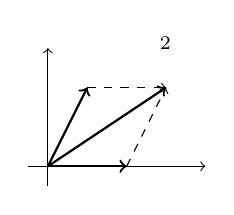
\begin{tikzpicture}
\draw[->] (0,-.25) -- (0,1.5);
\draw[->] (-.25,0) -- (2,0);

\draw (1.5,1.5) node{$\R^2$};

\draw[->, thick] (0,0) -- (.5,1);
\draw[->, thick] (0,0) -- (1,0);
\draw[->, dashed] (.5,1) -- (1.5,1);
\draw[->, dashed] (1,0) -- (1.5,1);
\draw[->, thick] (0,0) -- (1.5,1);
\end{tikzpicture}\qquad
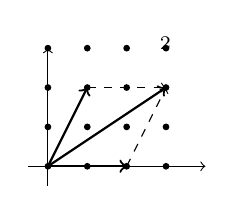
\begin{tikzpicture}
\draw[->] (0,-.25) -- (0,1.5);
\draw[->] (-.25,0) -- (2,0);

\foreach \x in {0,0.5,1,1.5}
	\foreach \y in {0,0.5,1,1.5}
		\filldraw (\x,\y) circle (1pt);

\draw (1.5,1.5) node{$\Z^2$};

\draw[->, thick] (0,0) -- (.5,1);
\draw[->, thick] (0,0) -- (1,0);
\draw[->, dashed] (.5,1) -- (1.5,1);
\draw[->, dashed] (1,0) -- (1.5,1);
\draw[->, thick] (0,0) -- (1.5,1);
\end{tikzpicture}
\end{center}
\end{bsp}

\section{Untergruppen und Gruppenhomomorphismen}

\begin{df}\label{2.2.1}[$\to$ \ref{1.1.12}]
Seien $(G,+_G)$ und $(H,+_H)$ abelsche Gruppen. Dann heißt $(H,+_H)$ eine \emph{Untergruppe}\index{abelsche Gruppe@{\bf abelsche Gruppe}!Untergruppe} von $(G,+_G)$, falls $H\subseteq G$ und $\forall a,b\in H:
a+_H b= a +_G b$.
\end{df}

\begin{pro}\label{2.2.2}
Sei $(G,+_G)$ eine abelsche Gruppe und $H$ eine Menge. Dann ist $H$ genau dann Trägermenge einer Untergruppe von $(G,+_G)$, wenn gilt:
\begin{enumerate}[\rm(a)]
\item $H\subseteq G$
\item $0_G \in H$
\item $\forall a,b \in H:a+_G b \in H$
\item $\forall a\in H:-_Ga\in H$
\end{enumerate}
In diesem Fall gibt es genau eine Abbildung $+_H:H\times H\rightarrow H$, mit der $(H,+_H)$ eine Untergruppe von $(G,+_G)$ wird.
Es gilt dann:
\begin{enumerate}
\item[\rm(b')] $0_H = 0_G$
\item[\rm(c')] $\forall a,b\in H:a+_H b = a+_G b$
\item[\rm(d')] $\forall a\in H:-_Ha = -_Ga$
\end{enumerate}
\end{pro}
\begin{proof}
Wir zeigen zunächst:
\[(*)\qquad((a)\et (b)\et (c)\et (d))\implies H\text{ ist Trägermenge einer Untergruppe von $(G,+_G)$.}\]
Gelte hierzu (a), (b), (c), (d). Definiere eine Abbildung
\[+_H:H\times H\rightarrow H, (a,b)\mapsto a+_G b\]
unter Ausnutzung von (a) und (c). Man sieht sofort, dass $(H,+_H)$ wegen (a) die Eigenschaften (K) und (A) aus
\ref{2.1.1} "`erbt"'. Gleiches gilt für $(N)$ und $(I)$ wegen (b) und (d). Damit ist $(*)$ gezeigt.

Für den Rest des Beweises sei $H$ Trägermenge einer Untergruppe von $(G,+_G)$.
Dann gibt es eine Gruppenaddition $+_H:H\times H\rightarrow H$ derart, dass $(H,+_H)$ eine Untergruppe von $(G,+_G)$ ist. Nach \ref{2.2.1} gelten (a) und (c'). Aus (c') folgt weiter, dass es \emph{genau} eine solche Gruppenaddition
gibt. Es bleiben nur noch (b') und (d') zu zeigen, denn (b') $\Longrightarrow$ (b), (c') $\Longrightarrow$ (c)
und (d') $\Longrightarrow$ (d).

\textbf{Zu (b').} Es gilt: $0_H+_G 0_H\overset{\text{(c')}}= 0_H+_H0_H\overset{\text{ (N) für }H}=0_H$.\\
Daraus folgt
\begin{multline*}
0_H\overset{\text{(N)}}{\underset{\text{für }G}=}0_H+_G 0_G
\overset{\text{(I)}}{\underset{\text{für }G}=}0_H+_G(0_H+_G(-_G0_H))\\
\overset{\text{(A)}}{\underset{\text{für }G}=}(0_H+_G0_H)+_G(-_G0_H)= 0_H +_G (-_G0_H)\overset{\text{(I)}}{\underset{\text{für }G}=}0_G.
\end{multline*}
\textbf{Zu (d').} Sei $a\in H$. Dann ist
$a+_G (-_H a) \overset{\text{(c')}}=a +_H (-_Ha)\overset{\text{(I)}}{\underset{\text{für }H}=}0_H
\overset{\text{(b')}}= 0_G$ und daher $-_Ha=-_Ga$ nach der Definition von $-_Ga$ in \ref{2.1.2}(b).
\end{proof}

\begin{bem}\label{2.2.3}
Ist $(H,+_H)$ eine Untergruppe der abelschen Gruppe $(G,+)$, so schreibt man wegen (b'), (c') und (d') fast immer $+,-,0$ statt $+_H,-_H,0_H$. Daher erwähnt man die Gruppenaddition oft nicht mehr explizit und spricht zum Beispiel von einer "`Untergruppe $H$ der (additiv geschriebenen) abelschen Gruppe $G$"'.
\end{bem}

\begin{bsp}\label{2.2.4}
\begin{enumerate}[\normalfont(a)]
\item Für jede abelsche Gruppe $G$ sind $\left\{0\right\}$ und $G$ (Trägermengen von) Untergruppen von $G$.
Für $\# G\leq 3$ besitzt $G$ keine weiteren Untergruppen.
Dies ist klar für $\#G\le2$, für $\#G\le3$ betrachte man die Additionstabelle aus \ref{2.1.3}(d).
\item Gelte $X\subseteq A$. Betrachte wieder die abelsche Gruppe $\Pow(A)$ mit $B+C=B\Delta C=(B\setminus C)\cup (C\setminus B)$. Es ist $H:=\left\{B\in\Pow(A)\mid B\cap X=\emptyset\right\}$ eine Untergruppe von $G$.
Hierzu ist zu zeigen: $H\subseteq\Pow(A)$, $0\in H$, $\forall B,C\in H:B+C\in H$ und $\forall B\in H:-B\in H$.
Wegen $0=\emptyset$ und $-B=B$ für $B\in H$ ist nur $(B\Delta C)\cap X=\emptyset$ für alle $B,C\in H$ zu zeigen, was
einfach ist.
\item Folgende Inklusionen sind Untergruppenbeziehungen:
\begin{gather*}
\left\{10n\mid n\in\Z\right\}\subseteq\begin{Bmatrix}\left\{5n\mid n\in \Z\right\}\\\left\{2n\mid n\in \Z\right\}\end{Bmatrix}\subseteq \Z\subseteq\begin{Bmatrix}\left\{\frac{n}{3}\mid n\in \Z\right\}\\\left\{\frac{n}{2}\mid n\in \Z\right\}\end{Bmatrix}\subseteq\left\{\frac{n}{6}\mid n\in \Z\right\}\subseteq \Q,\\
\Q\subseteq\left\{p+q\sqrt{2}\mid p,q\in\Q\right\}\subseteq\R,\\
\{(0,0)\}\subseteq\{(m,0)\mid m\in\Z\}\subseteq\{(m,2n)\mid m,n\in\Z\}\subseteq\Z\times\Z,\\
\Z\times\Z\subseteq\begin{Bmatrix}\Q\times\Z\\\Z\times\Q\end{Bmatrix}\subseteq\Q\times\Q\subseteq \Q\times\R\subseteq\R\times\R.
\end{gather*}
\item $\N_0$ ist \emph{keine} Untergruppe von $\Z$ bezüglich der (gewöhnlichen) Addition,
$(\Q\setminus \left\{0\right\},\cdot)$ ist \emph{keine} Untergruppe von $(\Q,+)$.
\end{enumerate}
\end{bsp}

\begin{pro}\label{2.2.5}
Sei $G$ eine abelsche Gruppe und $M$ eine Menge von Untergruppen von $G$. Dann ist auch $\bigcap M$ eine Untergruppe von $G$ (mit $\bigcap\emptyset:= G$) [$\to$ \ref{1.1.14}].
\end{pro}
\begin{proof}
Wir verwenden im Folgenden, dass
\[\bigcap M=\{a\in G\mid\forall I\in M:a\in I\},\]
was man sofort durch Fallunterscheidung nach den Fällen $M=\emptyset$ und $M\ne\emptyset$ zeigt.
Zu zeigen:
\begin{enumerate}[\normalfont(a)]
\item $\bigcap M\subseteq G$
\item $0\in \bigcap M$
\item $\forall a,b \in \bigcap M:a+b\in\bigcap M$
\item $\forall a\in\bigcap M:-a\in\bigcap M$
\end{enumerate}

\textbf{Zu (a).} \OE\ $M\neq \emptyset$. Sei $a\in\bigcap M$. Wähle $H\in M$ (beachte $M\ne\emptyset$). Dann
$a\in H\subseteq G$, also $a\in G$.

\textbf{Zu (b).} Sei $H\in M$. Zu zeigen: $0\in H$. Klar, da $H$ Untergruppe.

\textbf{Zu (c).} Seien $a,b\in \bigcap M$. Zu zeigen: $a+b\in\bigcap M$. Sei $H\in M$. Zu zeigen: $a+b\in H$.
Wissen $a,b\in H$. Da $H$ Untergruppe, folgt $a+b\in H$.

\textbf{Zu (d).} Sei $a\in\bigcap M$. Zu zeigen: $-a\in\bigcap M$. Sei $H\in M$. Zu zeigen: $-a\in H$. Wissen $a\in H$. Da $H$ Untergruppe, folgt $-a\in H$.
\end{proof}

\begin{satdef}\label{2.2.6}
Sei $G$ eine abelsche Gruppe und $E\subseteq G$. Dann existiert \underline{\underline{die}} \underline{kleinste}
Untergruppe $H$ von $G$ mit $E\subseteq H$. (d.h. $H$ ist eine Untergruppe von $G$ mit $E\subseteq H$ und wenn
$H'$ auch eine solche ist, so gilt $H\subseteq H'$). Man nennt sie die von $E$ in $G$ \emph{erzeugte} Untergruppe\index{abelsche Gruppe@{\bf abelsche Gruppe}!Untergruppe!erzeugte Untergruppe} von $G$ und notiert sie mit $\langle E\rangle_G$.
\end{satdef}
\begin{proof}
Für $M:=\{I\mid I\text{ Untergruppe von }G,E\subseteq I\}$ ist
$H:=\bigcap M$ ist eine Untergruppe von $G$ nach \ref{2.2.5}. Offensichtlich gilt $E\subseteq H$.
Schließlich ist $H\subseteq H'$ zu zeigen für alle $H'\in M$. Dies ist aber trivial wegen $H=\bigcap M$.
\end{proof}

\begin{sat}\label{2.2.7}
Sei $G$ eine abelsche Gruppe und $E\subseteq G$. Dann
$$\langle E\rangle_G = \Set{\sum_{i=1}^{m}a_i-\sum_{i=1}^{n}b_i | m,n\in\N, a_1,\ldots,a_m,b_1,\ldots,b_n\in E}$$
\end{sat}
\begin{proof}(gleichzeitig alternativer Beweis für Satz \ref{2.2.6}!)
Man überlegt sich leicht, dass die rechtsstehende Menge eine Untergruppe von $G$ ist, die $E$ enthält. Sei $H$ eine
weitere Untergruppe von $G$ mit $E\subseteq H$. Zu zeigen ist, dass die rechtsstehende Menge in $H$ enthalten ist,
was aber trivial ist.
\end{proof}

\begin{bsp}\label{2.2.8}
$\langle \left\{3,2\right\}\rangle_\Z = \Z$, $\langle\{12,16\}\rangle_\Z=\{4n\mid n\in\Z\}$
\end{bsp}

\begin{df}\label{2.2.9}
Seien $(G,+_G)$ und $(H,+_H)$ abelsche Gruppen. Dann heißt $f$ ein \mbox{(Gruppen-)}Homo\-morphismus von $(G,+_G)$ nach
$(H,+_H)$, wenn $f\colon G\to H$ eine Abbildung ist mit \[\forall a,b\in G: f(a+_Gb)=f(a)+_Hf(b).\]
\end{df}

\begin{ged}\label{2.2.10}
Idee eines Homomorphismus: "`erst rechnen dann abbilden"' ist dasselbe wie "`erst abbilden dann rechnen"'.
\end{ged}

\begin{pro}\label{2.2.11}
Seien $(G,+_G)$ und $(H,+_H)$ abelsche Gruppen und sei $f$ ein Homomorphismus von
$(G,+_G)$ nach $(H,+_H)$. Dann gilt $f(0_G)=0_H$ und $f(-_G a)=-_Hf(a)$ für alle $a\in G$.
\end{pro}
\begin{proof}
Aus $0_G=0_G +_G 0_G$ folgt $f(0_G)=f(0_G +_G 0_G)\overset{\text{$f$ Hom.}}=f(0_G) +_H f(0_G)$ und daher $0_H = f(0_G) -_H f(0_G) = f(0_G) +_H f(0_G) -_H f(0_G)=f(0_G)$.

Sei nun $a\in G$. Um $f(-_G a) = -_H f(a)$ zu zeigen, ist $f(a)+_H f(-_G a) = 0_H$ zu zeigen.
Nun gilt aber $f(a)+_H f(-_G a)= f(a +_G (-_G a)) = f(0_G) = 0_H$.
\end{proof}

\begin{nt}\label{2.2.12}[$\to$ \ref{1.1.29}(c)]
Ein Gruppenhomomorphismus $f:G\rightarrow H$ heißt
(Gruppen-)$\begin{Bmatrix}\text{\emph{Einbettung oder Mono-}}\\\text{\emph{Epi-}}\\\text{\emph{Iso-}}\end{Bmatrix}$ \emph{morphismus}\index{abelsche Gruppe@{\bf abelsche Gruppe}!Homomorphismus!Isomorphismus}\index{abelsche Gruppe@{\bf abelsche Gruppe}!Homomorphismus!Monomorphismus}\index{abelsche Gruppe@{\bf abelsche Gruppe}!Homomorphismus!Epimorphismus}, wenn $f\begin{Bmatrix}\text{injektiv}\\\text{surjektiv}\\\text{bijektiv}\end{Bmatrix}$ ist.
Einen Gruppenhomomorphismus $f:G\rightarrow G$ nennt man auch einen (Gruppen-)\emph{Endomorphismus} von $G$\index{abelsche Gruppe@{\bf abelsche Gruppe}!Homomorphismus!Endomorphismus} und, falls er bijektiv ist,
(Gruppen-)\emph{Automorphismus}\index{abelsche Gruppe@{\bf abelsche Gruppe}!Homomorphismus!Automorphismus} von $G$.
\end{nt}

\begin{bsp}\label{2.2.13}
\[
\begin{array}{r|c|c|c|c|c|c}
 &\text{Hom.}&\text{Einb.}&\text{Epi.}&\text{Iso.}&\text{Endo.}&\text{Auto.}\\\hline
 \Z\rightarrow\Z, a\mapsto 2a & \checkmark & \checkmark & \text{---} & \text{---} & \checkmark & \text{---} \\\hline
 \Z\rightarrow\Q, a\mapsto 2a & \checkmark & \checkmark & \text{---} & \text{---} & \text{---} & \text{---} \\\hline
 \Q\rightarrow \Q, a\mapsto 2a & \checkmark & \checkmark & \checkmark & \checkmark & \checkmark & \checkmark \\\hline
 \Z\rightarrow \Z, a\mapsto-a & \checkmark & \checkmark & \checkmark & \checkmark & \checkmark & \checkmark \\\hline
 \Z\times\Z\rightarrow \Z, (a,b)\mapsto a & \checkmark & \text{---} & \checkmark & \text{---} & \text{---} & \text{---} \\\hline
  \Z\times\Z\rightarrow \Z, (a,b)\mapsto a+b& \checkmark & \text{---} & \checkmark & \text{---} & \text{---} & \text{---} \\\hline
\Z\rightarrow \Z, a\mapsto a+1 & \text{---} & \text{---} & \text{---} & \text{---} & \text{---} & \text{---} \\\hline
\Z\to\Z\times\Z, a\mapsto(a,a) & \checkmark & \checkmark &  \text{---} & \text{---} & \text{---} & \text{---}\\\hline
\Z\to\Z\times\Z, a\mapsto(a,0) & \checkmark & \checkmark &  \text{---} & \text{---} & \text{---} & \text{---}\\\hline
\underset{{\tiny\text{(jeweils mit Multiplikation)}} }{\R\setminus\left\{0\right\}\rightarrow \R_{>0},}a\mapsto |a|& \checkmark & \text{---} & \checkmark & \text{---} & \text{---} & \text{---}
\end{array}
\]
\end{bsp}

\begin{pro}\label{2.2.14}
\begin{enumerate}[\rm(a)]
\item Seien $G,H,I$ abelsche Gruppen. Sind $G\overset{f} \rightarrow H\overset{g}\rightarrow I$ Gruppenhomomorphismen, so auch $g\circ f$.
\item Ist $f:G\rightarrow H$ ein Gruppenisomorphismus, so auch $f^{-1}$.
\end{enumerate}
\end{pro}
\begin{proof}
(a)
Seien $G\overset{f} \rightarrow H\overset{g}\rightarrow I$ Gruppenhomomorphismen und $a,b\in G$. Dann
\begin{multline*}
(g\circ f)(a+b)=g(f(a+b))\overset{f\text{ Hom.}}=g(f(a)+f(b))
\overset{g\text{ Hom.}}=g(f(a)) + g(f(b))\\= (g\circ f)(a)+(g\circ f)(b).
\end{multline*}

(b) Sei $f:G\rightarrow H$ ein Gruppenisomorphismus. Nach \ref{1.2.5}(d) ist $f^{-1}$ bijektiv. Es ist noch zu zeigen, dass $f^{-1}$ ein Homomorphismus ist. Seien hierzu $a,b\in H$. Da $f$ injektiv ist, reicht es
 $f(f^{-1}(a+b))=f(f^{-1}(a)+f^{-1}(b))$ zu zeigen. Es gilt aber
$f(f^{-1}(a+b))=(f\circ f^{-1})(a+b)\overset{\ref{1.2.5}(c)}=\id_H(a+b)=a+b$
und $f(f^{-1}(a)+f^{-1}(b)) \overset{f\text{ Hom.}}= f(f^{-1}(a))+f(f^{-1}(b))
=(f\circ f^{-1})(a)+(f\circ f^{-1})(b)=\id_H(a)+\id_H(b)=a+b$.
\end{proof}

\red{Bis hierher sollten wir am 11. November kommen.}

\begin{defbem}\label{2.2.15}
Zwei abelsche Gruppen $G$ und $H$ heißen \emph{isomorph}\index{abelsche Gruppe@{\bf abelsche Gruppe}!isomorph ($\cong$)}, wenn es einen Isomorphismus von $G$ nach $H$ gibt, in Zeichen $G\cong H$.\\
Ein Gruppenisomorphismus führt also die Additionstabelle der einen abelschen Gruppe in eine Additionstabelle der anderen abelschen Gruppe über:
\begin{table}[h!]
\centering
\begin{tabular}{c|ccc}
$+$ & $\cdots$ & $b$ & $\cdots$ \\\hline
$\vdots$ & & $\vdots$ &\\
$a$ & $\dotsm$ & $a+b$ & $\dotsm$ \\
$\vdots$ & & $\vdots$ &
\end{tabular}
\qquad$\leadsto$\qquad
\begin{tabular}{c|ccc}
$+$ & $\cdots$ & $f(b)$ & $\cdots$\\\hline
$\vdots$ & & $\vdots$ &\\
$f(a)$ & $\dotsm$ &$f(a+b)$ & $\dotsm$ \\
$\vdots$ & & $\vdots$ &
\end{tabular}
\end{table}\\
Er tauscht die Elemente aus, ohne die "`Gruppenstruktur"' zu verändern
(das heißt die über die Addition geregelten Beziehungen der Elemente untereinander). Alle "`strukturellen"' (das heißt
nicht auf die Natur der Elemente bezogenen) Eigenschaften einer abelschen Gruppe übertragen sich daher unter Isomorphismen. Dass zwei abelsche Gruppen isomorph sind, heißt, dass ihre Additionstabellen dieselbe Form haben.
\end{defbem}

\begin{bsp}\label{2.2.16}
\begin{enumerate}[\normalfont(a)]
\item Seien $(G,+_G)$ und $(H,+_H)$ abelsche Gruppen mit $\# G = 3 = \# H$. Nach \ref{2.1.3}(d) kann man dann
 $a,b,c,d$ mit $G=\{0_G,a,b\}$ und $H=\{0_H,c,d\}$ finden so, dass die Additionstabellen von $(G,+_G)$ und $(H,+_H)$
 wie folgt lauten:
\begin{table}[h!]
\centering
\begin{tabular}{c|ccc}
$+_G$ & $0_G$ & $a$ & $b$ \\\hline
$0_G$ & $0_G$ & $a$ & $b$ \\
$a$ & $a$ & $b$ & $0_G$ \\
$b$ & $b$ & $0_G$ & $a$
\end{tabular}
\qquad\text{und}\qquad
\begin{tabular}{c|ccc}
$+_H$ & $0_H$ & $c$ & $d$ \\\hline 
$0_H$ & $0_H$ & $c$ & $d$ \\ 
$c$ & $c$ & $d$ & $0_H$ \\
$d$ & $d$ & $0_H$ & $c$
\end{tabular} 
\end{table}\\
Daher ist $f:G\rightarrow H,\ \begin{array}[c]{c}0_G\mapsto 0_H\\a\mapsto c\\b\mapsto d\end{array}$ ein Isomorphismus von
$(G,+_G)$ nach $(H,+_H)$, also $(G,+_G)\cong(H,+_H)$.
Man sagt, dass es "`\emph{bis auf Isomorphie}"' genau eine dreielementige abelsche Gruppe gibt.
Dasselbe gilt nach \ref{2.1.3} für ein- und zweielementige abelsche Gruppen.
\item Sei $G$ eine abelsche Gruppe mit $\#G\le3$. Ist $\#G\le2$, so ist $\id_G$ der einzige Automorphismus von $G$
(für $\#G=2$ folgt dies aus \ref{2.2.11}). Ist $\#G=3$, so gibt es genau zwei Automorphismen von $G$, wie man an der
Additionstabelle in \ref{2.1.3}(d) leicht erkennt: $\id_G$ und die Permutation von $G$, die die zwei nichtneutralen Elemente vertauscht.
\end{enumerate}
\end{bsp}

\begin{spr}\label{2.2.17}
"`Isomorphismus $=$ Umbenennung der Elemente"'\index{abelsche Gruppe@{\bf abelsche Gruppe}!Homomorphismus!Isomorphismus}
\end{spr}

\section[tocentry={Quotientengruppen}]{Quotientengruppen{\small [$\to$ §\ref{1.3}]}}\label{2.3}

\noindent
Idee: Grobe Sichtweise auf eine abelsche Gruppe einnehmen.

\begin{df} \label{2.3.1}
Sei $G$ eine abelsche Gruppe. Eine \emph{Kongruenzrelation}\index{Relation@{\bf Relation}!Kongruenzrelation ($\equiv$)} auf $G$ ist eine Äquivalenzrelation $\equiv$ auf $G$, für die gilt:
\begin{equation}\tag{$*$}\label{star1}
\forall a,a',b,b'\in G:((a\equiv a' ~\et~ b\equiv b')\implies a+b\equiv a'+b')
\end{equation}
Für $a\in G$ nennt man $\overline a:=\overset\equiv a$ ("`ein Strich gleich drei Strich"'-Regel zur Vereinfachung der Notation!) statt Äquivalenz- auch \emph{Kongruenzklasse}\index{Relation@{\bf Relation}!Kongruenzrelation ($\equiv$)!Kongruenzklasse} von $a$ bezüglich $\equiv$.
\end{df}

\begin{bem}\label{2.3.2}
In Definition \ref{2.3.1} drückt Bedingung \eqref{star1} gerade folgendes aus:
\begin{equation}\tag{$**$}\label{starstar}
\begin{aligned}
G/\mbox{$\equiv$}~\times~G/\mbox{$\equiv$}~ & \to~G/\mbox{$\equiv$}\\
(\overline a,\overline b) & \mapsto\overline{a+b}\quad(a,b\in G)
\end{aligned}
\quad
\text{ ist wohldefiniert.}
\end{equation}
In der Tat: $\eqref{starstar}\iff(\forall a,b,a',b'\in G:((\overline a,\overline b)=(\overline{a'},\overline{b'})\implies\overline{a+b}=\overline{a'+b'}))\iff\eqref{star1}.$
\end{bem}

\begin{satdef}\label{2.3.3}
Sei $G$ eine abelsche Gruppe und $\equiv$ eine Kongruenzrelation auf $G$. Dann wird die Quotientenmenge $G/\mbox{$\equiv$}$ vermöge der durch
$$\overline a+\overline b:=\overline{a+b}\qquad(a,b\in G)$$
festgelegten ("`vertreterweisen"') Addition zu einer abelschen Gruppe, die man die zu $\equiv$ gehörige \emph{Quotientengruppe}\index{Relation@{\bf Relation}!Kongruenzrelation ($\equiv$)!Quotientengruppe} von $G$
nennt (auch "`$G$ nach $\equiv$"' oder "`$G$ modulo $\equiv$"'). In ihr gilt $0=\overline0$ und $-\overline a=\overline{-a}$ für alle $a\in G$.
\end{satdef}
\begin{proof}
Die Wohldefiniertheit der Addition auf $A/\mbox{$\equiv$}$ als Abbildung haben wir schon in Bemerkung \ref{2.3.2} geklärt. Wir prüfen die Axiome (K), (A), (N) und (I) aus
\ref{2.1.1} nach:
\begin{enumerate}
\item[(K)] $\overline a+\overline b=\overline{a+b}=\overline{b+a}=\overline b+\overline a$ für alle $a,b\in G$.
\item[(A)]  $(\overline a+\overline b)+\overline c=\overline{a+b}+\overline c=\overline{(a+b)+c}=\overline{a+(b+c)}=\overline a+\overline{b+c}=
\overline a+(\overline b+\overline c)$ für alle $a,b,c\in G$.
\item[(N)] Für $a\in G$ gilt $\overline a+\overline0=\overline{a+0}=\overline a$. Daher ist $0=\overline 0$.
\item[(I)] Für $a\in G$ gilt $\overline a+\overline{-a}=\overline{a+(-a)}=\overline0=0$. Daher ist $-\overline a=\overline{-a}$ für $a\in G$.
\end{enumerate}
\end{proof}

\begin{pro}\label{2.3.4}
Sei $G$ eine abelsche Gruppe und $\equiv$ eine Kongruenzrelation auf $G$. Dann ist $H:=\overline0$ eine Untergruppe von $G$, für die gilt:
\begin{enumerate}[\rm(a)]
\item $\forall a,b\in G:(a\equiv b\iff a-b\in H)$
\item $\forall a\in G:\overline a=\{a+b\mid b\in H\}$ \label{hpropb}
\item Für jedes $a\in G$ ist $H\to\overline a,\ b\mapsto a+b$ bijektiv. \label{hpropc}
\end{enumerate}
\end{pro}
\begin{proof}
Um zu zeigen, dass $H$ eine Untergruppe von $G$ ist, sind nach Proposition \ref{2.2.2} zeigen:
\begin{enumerate}[(1)]
\item $H\subseteq G$
\item $0\in H$
\item $\forall a,b\in H:a+b\in H$
\item $\forall a\in H:-a\in H$
\end{enumerate}
(1) und (2) sind trivial. Um (3) zu sehen, beobachten wir, dass für alle $a,b\in H$ wegen $a\equiv0$ und $b\equiv0$ aus \eqref{star1} folgt
$a+b\equiv0+0=0$ und daher $a+b\in H$.  Schließlich erhält man (4) daraus, dass für alle $a\in H$ aus $a\equiv0$ und $-a\equiv-a$ gemäß \eqref{star1}
$0=a-a\equiv0-a=-a$ und damit $-a\equiv0$ folgt.

\smallskip
{\bf (a)} Seien $a,b\in G$. Gilt $a\equiv b$, so wegen $-b\equiv-b$ gemäß \eqref{star1} auch $a-b\equiv b-b=0$ und daher $a-b\in\overline0=H$. Gilt umgekehrt $a-b\in H$, so
$a-b\equiv0$ und wegen $b\equiv b$ gemäß \eqref{star1} auch $a=a-b+b\equiv b$.

\smallskip
{\bf (b)} Sei $a\in G$. Wir behaupten $\overline a=\{a+b\mid b\in H\}$.

"`$\subseteq$"' Ist $c\in\overline a$, so gilt $c\equiv a$, woraus mit \eqref{star1} folgt $b:=c-a\equiv a-a=0$ und $c=a+b$.

"`$\supseteq$"' Ist umgekehrt $b\in\overline0$, so folgt mit \eqref{star1}, dass $a+b\equiv a+0=a$ und damit $a+b\in\overline a$.

\smallskip
{\bf (c)} Die Surjektivität ist gerade (b), die Injektivität ist leicht zu zeigen.
\end{proof}

\begin{df}\mbox{}[$\to$ \ref{1.3.5}(b)]\label{2.3.5}
Sei $G$ eine abelsche Gruppe. Zu jeder Untergruppe $H$ von $G$ definieren wir eine Relation $\equiv_H$ auf $G$ durch
$$a\equiv_H b:\iff a-b\in H.$$\index{Relation@{\bf Relation}!Kongruenzrelation ($\equiv$)!h@$\equiv_H$}
\end{df}

\begin{sat}\text{\rm[$\to$\ref{1.3.6}]} \label{2.3.6} Sei $G$ eine abelsche Gruppe. Die Zuordnungen
\begin{align*}
\equiv&\mapsto\overline0\\
\equiv_H&\mapsfrom H
\end{align*}
vermitteln eine Bijektion zwischen der Menge der Kongruenzrelationen auf $G$ und der Menge der Untergruppen von $G$.
\end{sat}
\begin{proof}
Zu zeigen ist:
\begin{enumerate}[\normalfont(a)]
\item Ist $\equiv$ eine Kongruenzrelation auf $G$, so ist $\overline0$ eine Untergruppe von $G$.
\item Ist $H$ eine Untergruppe von $G$, so ist $\equiv_H$ eine Kongruenzrelation auf $G$.
\item Ist $\equiv$ eine Kongruenzrelation auf $G$, so $\equiv_{\overline0}~=~\equiv$.
\item Ist $H$ eine Untergruppe von $G$, so $\overset{-_H}0=H$.
\end{enumerate}
\medskip\noindent
{\bf (a)} wurde bereits in Proposition \ref{2.3.4} gezeigt. 

\medskip\noindent
{\bf Zu (b).} Sei $H$ eine Untergruppe von $G$. Zu zeigen ist, dass $\equiv_H$ eine Äquivalenzrelation ist [$\to$ \ref{1.3.1}] und dass $(*)$ aus \ref{2.3.2} gilt. Also ist zu zeigen:
\begin{enumerate}[(1)]
\item $\forall a\in G:a\equiv_H a$
\item $\forall a,b\in G:(a\equiv_Hb\implies b\equiv_Ha)$
\item $\forall a,b,c\in G:((a\equiv_Hb~\&~b\equiv_Hc)\implies a\equiv_H c)$
\item $\forall a,a',b,b'\in G:((a\equiv_Ha'\et b\equiv_Hb')\implies a+b\equiv_Ha'+b')$.
\end{enumerate}

Zu (1). Ist $a\in G$, dann $a-a=0\in H$ und damit $a\equiv_H a$.

Zu (2). Seien $a,b\in G$ mit $a\equiv_Hb$. Dann $a-b\in H$ und daher $b-a=-(a-b)\in H$. Also $b\equiv_Ha$.

Zu (3). Seien $a,b,c\in G$ mit $a\equiv_Hb$ und $b\equiv_Hc$. Dann $a-b\in H$ und $b-c\in H$. Also $a-c=(a-b)+(b-c)\in H$.

Zu (4). Seien $a\equiv_Ha'$ und $b\equiv_Hb'$. Dann $a-a'\in H$ und $b-b'\in H$. Also $a+b-(a'+b')=(a-a')+(b-b')\in H$, das heißt $a+b\equiv_Ha'+b'$.

\medskip\noindent
{\bf Zu (c).} Seien $\equiv$ eine Kongruenzrelation auf $G$ und $a,b\in G$. Zu zeigen ist $a\equiv_{\overline0}b\iff a\equiv b$. Dies sieht man leicht:
$$a\equiv_{\overline0}b\overset{\ref{2.3.5}}\iff a-b\in\overline0\overset{\text{\ref{1.3.1}(b)}}\iff a-b\equiv0\overset{(*)}\iff a\equiv b.$$

\medskip\noindent
{\bf Zu (d).} Ist $H$ eine Untergruppe von $G$, so  $$\overset{-_H}0\overset{\text{\ref{1.3.1}(b)}}=\{a\in G\mid a\equiv_H0\}\overset{\ref{2.3.5}}=\{a\in G\mid a-0\in H\}=H.$$
\end{proof}

\begin{notsprpro}\label{2.3.7}
Sei $H$ eine Untergruppe der abelschen Gruppe $G$. Dann nennt man $G/H:=G/\mbox{$\equiv_H$}$ die \emph{Quotientengruppe}\index{Relation@{\bf Relation}!Kongruenzrelation ($\equiv$)!Quotientengruppe} von $G$ nach (oder modulo) $H$.
Die Kongruenzklassen $\overset{-_H}{a~}$ ($a\in G$) {\rm[$\to$ \ref{2.3.1}]} von $\equiv_H$ nennen wir auch die \emph{Nebenklassen}\index{Relation@{\bf Relation}!Kongruenzrelation ($\equiv$)!Nebenklassen} von $H$ (in $G$).
Wegen \ref{2.3.4}\eqref{hpropc} haben alle Nebenklassen von $H$ dieselbe Mächtigkeit  {\rm[$\to$ \ref{1.1.21}]} und da sie eine Zerlegung {\rm[$\to$ \ref{1.3.3}]}
von $G$ bilden, gilt
$$\#G=(\#(G/H))(\#H),$$
falls $G$ endlich ist, denn $\#(G/H)$ ist dann die Anzahl der Nebenklassen von $H$ und jede Nebenklasse von $H$ hat $\#H$ viele Elemente.
\end{notsprpro}

\begin{bsp}\label{2.3.8}
Sei $G$ eine abelsche Gruppe.
\begin{enumerate}[\normalfont(a)]
\item $G/G=\{G\}=\{0\}$ ist einelementig.
\item Es gilt $G/\{0\}=\{\{a\}\mid a\in G\}$, wobei $\{a\}+\{b\}=\{a+b\}$ für alle $a,b\in G$ gilt. Man sieht sofort, dass $G\to G/\{0\},\ a\mapsto\{a\}$ ein Isomorphismus ist.
Insbesondere gilt $G/\{0\}\cong G$.
\end{enumerate}
\end{bsp}

\begin{bsp}\label{2.3.9}
Sei $n\in\Z$. Die von $\{n\}$ erzeugte Untergruppe von $\Z$ ist $\langle n\rangle:=\langle\{n\}\rangle_\Z=\{cn\mid c\in\Z\}$. Es gilt
$$\Z/\langle n\rangle=\left\{\overset{-_{\langle n\rangle}}{a~~~}\mid a\in\Z\right\},\quad\text{ wobei}$$
$$\overset{-_{\langle n\rangle}}{a~~~}=\overset{-_{\langle n\rangle}}{b~~~}\iff
a\equiv_{\langle n\rangle}b\iff a-b\in\langle n\rangle\iff\exists c\in\Z:a-b=cn.$$

[Zeichne Bild!]

Man überlegt sich sofort: Ist $n\in\N$, so hat $\Z/\langle n\rangle$ genau $n$ Elemente und es gilt
$$\Z/\langle n\rangle=\left\{\overset{-_{\langle n\rangle}}{0~~~},\overset{-_{\langle n\rangle}}{1~~~},\dots,\overset{\text{---------}_{\langle n\rangle}}{n-1~~~}\right\}.$$
Ist $n=0$, so ist $Z/\langle0\rangle=\{\{a\}\mid a\in\Z\}\cong\Z$. Ist $-n\in\N$, so gilt $\langle n\rangle=\langle-n\rangle$ und daher
$\Z/\langle n\rangle=\Z/\langle-n\rangle$.
\end{bsp}

\begin{defprop}\label{2.3.10}
Seien $G$ und $H$ abelsche Gruppen und $f\colon G\to H$ ein Homomorphismus.
\begin{enumerate}[\normalfont(a)]
\item Es ist $\equiv_f~:=~\sim_f$ [$\to$\ref{1.3.9}] eine Kongruenzrelation auf $G$.
\item Es ist der \emph{Kern}\index{Abbildung@{\bf Abbildung}!Kern ($\ker$)} $\ker f:=f^{-1}(\{0\})$ [$\to$\ref{1.1.25}] von $f$ eine Untergruppe von $G$.
\item Unter der Bijektion aus Satz \ref{2.3.6} entsprechen sich $\equiv_f$ und $\ker f$, das heißt
$$\ker f=\overset{-_f}{0~}\qquad\text{und}\qquad\equiv_f~=~\equiv_{\ker f}.$$
\end{enumerate}
\end{defprop}
\begin{proof}
{\bf (a)} Seien $a,a',b,b'\in G$ mit $a\equiv_f a'$ und $b\equiv_f b'$. Zu zeigen ist $a+b\equiv_f a'+b'$. Nach Definition von $\equiv_f~=~\sim_f$ in \ref{1.3.9} gilt
$f(a)=f(a')$ und $f(b)=f(b')$ und es ist $f(a+b)=f(a'+b')$ zu zeigen. Dies ist aber klar, denn
$$f(a+b)\overset{\ref{2.2.9}}=f(a)+f(b)=f(a')+f(b')\overset{\ref{2.2.9}}=f(a'+b').$$

\smallskip\noindent
{\bf (b)} Nach \ref{2.2.2} ist zu zeigen:
$$\ker f\subseteq G,\quad 0\in\ker f,\quad \forall a,b\in\ker f:a+b\in\ker f\quad\text{ und }\quad\forall a\in\ker f:-a\in\ker f.$$
Trivial ist $\ker f\subseteq G$, da $f^{-1}(\{0\})$ natürlich in der Definitionsmenge $G$ von $f$ enthalten ist. Die Bedingung $0\in\ker f$ entspricht genau der Beobachtung $f(0)=0$ aus \ref{2.2.11}. Sind $a,b\in\ker f$, dann
gilt $f(a)=0=f(b)$ und daher $f(a+b)=f(a)+f(b)=0+0=0$, also $a+b\in\ker f$. Ist schließlich $a\in\ker f$, also $f(a)=0$, so gilt $f(-a)\overset{\ref{2.2.11}}=-f(a)=-0\overset{0+0=0}=0$ und
daher $-a\in\ker f$.

\smallskip\noindent
{\bf (c)} Wegen Satz \ref{2.3.6} sind die beiden Gleichheiten äquivalent. Es reicht daher eine der beiden zu zeigen. Wir zeigen die erste. Diese ergibt sich wie folgt:
\begin{multline*}
\ker f\overset{(b)}=f^{-1}(\{0\})\overset{\ref{1.1.25}}=\{a\in G\mid f(a)=0\}\overset{\ref{2.2.11}}=\{a\in G\mid f(a)=f(0)\}\overset{\ref{1.3.9}}=\\\{a\in G\mid a\equiv_f0\}\overset{\ref{1.3.1}(b)}=
\overset{-_f}{0~}.
\end{multline*}
\end{proof}

\red{Bis hierher sollten wir am 15. November kommen.}

\begin{sat}[Homomorphiesatz für abelsche Gruppen]\label{2.3.11}{\rm[$\to$\ref{1.3.8}]}
Seien $G$ und $H$ abelsche Gruppen, $I$ eine Untergruppe von $G$ und $f\colon G\to H$ ein Homomorphismus
mit $I\subseteq\ker f$.
\begin{enumerate}[\rm(a)]
\item
Es gibt genau eine Abbildung $\overline f\colon G/I\to H$ mit
$\overline f(\overset{-_I}a)=f(a)$ für alle $a\in G$. Diese Abbildung $\overline f$ ist ein Homomorphismus.
\item
$\text{$\overline f$ ist injektiv}\iff I=\ker f$
\item
$\text{$\overline f$ ist surjektiv}\iff\text{$f$ ist surjektiv.}$
\end{enumerate}
\end{sat}
\begin{proof}
Nach Satz \ref{2.3.6} (genauer der Wohldefiniertheit der dortigen Abbildung von rechts nach links) ist $\equiv_I$ eine Kongruenzrelation auf $G$. Aus der Voraussetzung
$I\subseteq\ker f$ erhält man
$$a\equiv_Ib\implies f(a)=f(b)$$
für alle $a,b\in G$, denn sind $a,b\in G$ mit $a\equiv_Ib$, so  $a-b\in I\subseteq\ker f$ nach Definition \ref{2.3.5} und damit
$f(a)-f(b)\overset{\text{$f$ Hom.}}=f(a-b)=0$. Unter Beachtung von $G/I\overset{\ref{2.3.7}}=G/\mbox{$\equiv_I$}$ erhält man die in (a) behauptete
Existenz und Eindeutigkeit der Abbildung $\overline f$ daher aus dem Homomorphiesatz für Mengen \ref{1.3.8}. Dass $\overline f$ ein Homomorphismus ist, rechnet man sofort nach:
$$\overline f(\overset{-_I}a)+\overline f(\overset{-_I}b)\overset{(a)}=f(a)+f(b)\overset{\text{$f$ Hom.}}=f(a+b)=\overline f(\overset{\text{---------}_I}{a+b~~})\overset{\ref{2.3.3}}=
\overline f(\overset{-_I}a+\overset{-_I}b)$$
für alle $a,b\in G$. Damit ist (a) gezeigt. Die Aussage (c) folgt direkt aus \ref{1.3.8}(c). Schließlich ist es eine leichte Übung zu zeigen, dass die Aussage $I=\ker f$ äquivalent ist zu
$\forall a,b\in G:(a\equiv_Ib\iff f(a)=f(b))$, womit (b) nichts anderes als \ref{1.3.8}(b) ist.
\end{proof}

\begin{bem}{\rm[$\to$\ref{1.3.10}]}\label{2.3.12}
Sei $I$ eine Untergruppe einer abelschen Gruppe $G$. Dann wird $I$ durch einen Gruppenhomomorphismus
$f\colon G\to H$ in eine weitere abelsche Gruppe $H$ induziert, nämlich durch den \emph{kanonischen Epimorphismus}\index{abelsche Gruppe@{\bf abelsche Gruppe}!Homomorphismus!kanonischer Epimorphismus} [$\to$\ref{2.2.12}]
$$f\colon G\to G/I,\ a\mapsto\overset{-_I}a.$$
In der Tat: $\ker f=\{a\in G\mid f(a)=0\}=\{a\in G\mid \overset{-_I}a=0\}=\{a\in G\mid a\in I\}=I$.
\end{bem}

\begin{notpro}\label{2.3.13}
Seien $G$ und $H$ abelsche Gruppen und $f\colon G\to H$ ein Homomorphismus. Dann schreiben wir meist $\im f:=f(G)\overset{\ref{1.1.25}}=\{f(a)\mid a\in G\}$
für das in {\rm\ref{1.1.29}(d)} eingeführte Bild von $f$. Es ist $\im f$ eine Untergruppe von $H$.
\end{notpro}
\begin{proof}
Zu zeigen sind gemäß \ref{2.2.2}:
\begin{enumerate}[\normalfont(a)]
\item $\im f\subseteq H$
\item $0\in\im f$
\item $\forall a,b\in\im f:a+b\in\im f$
\item $\forall a\in\im f:-a\in\im f$
\end{enumerate}
(a) ist trivial und (b) folgt aus $f(0)\overset{\ref{2.2.11}}=0$. Sind $a,b\in\im f$, so gibt es $c,d\in G$ mit $f(c)=a$ und $f(d)=b$, woraus $f(c+d)\overset{\text{$f$ Hom.}}=f(c)+f(d)=a+b$
und damit $a+b\in\im f$ folgt. Dies zeigt (c). Ist schließlich $a\in\im f$, so gibt es $c\in G$ mit $f(c)=a$, woraus $f(-c)\overset{\ref{2.2.11}}=-f(c)=-a$ und damit $-a\in\im f$ folgt. Damit haben wir auch (d) gezeigt und sind fertig.
\end{proof}

\begin{kor}[Isomorphiesatz für abelsche Gruppen]\label{2.3.14} {\rm[$\to$\ref{1.3.11}]}
Seien $G$ und $H$ abelsche Gruppen und $f\colon G\to H$ ein Homomorphismus.
Dann ist $\overline f\colon G/\ker f\to\im f$
definiert durch $\overline f(\overset{-_{\ker f}}{a~~})=f(a)$ für $a\in G$ ein Isomorphismus {\rm[$\to$\ref{2.2.12}]}. Insbesondere $G/\ker f\cong\im f$ {\rm[$\to$\ref{2.2.15}]}.
\end{kor}

\begin{bem}\label{2.3.15}
Der Isomorphiesatz klärt uns über die Natur von Homomorphismen auf:
\begin{center}
\begin{tikzpicture}
 \node(G){$G$};
 \node[right = 4cm of G](H){$H$};
 \node[below = 2cm of G](Gkerf){$G/\ker f$};
 \node[below = 2cm of H](imf){$\im f$};
 
 \draw[->, thick] (G) -- node[above]{$f$ Hom.} (H);
 \draw[->, thick] (G) -- node[anchor = north, rotate = -90]{kan. Epi.} node[anchor = south, rotate = -90]{$a\mapsto \overset{\text{---}_{\ker f}}{a~~~~~}$} node[left](l){} (Gkerf);
 \draw[->, thick] (Gkerf) -- node[above](u){Iso.} (imf);
 \draw[->, thick] (H) -- node[anchor = south, rotate = 90]{$\subseteq$} node[anchor = north, rotate = 90]{Untergr.} node[right](r){} (imf);
 
 \node[left =.5 of l]{$I$};
 \node[below =.5 of u]{$II$};
 \node[right =.5 of r]{$III$};
 
 \draw[->, thick] (2.15,-.75) arc (125:425:.5);
\end{tikzpicture}
\end{center}
Drei Phasen:
$$G\xrightarrow[\text{"`vergröbern"'}]{I} G/\ker f\xrightarrow[\text{"`umbenennnen"'}]{II}\im f\xrightarrow[\text{"`neue Elemente dazufügen"'}]{III}H$$
\end{bem}

\end{document}